\documentclass{article}

\usepackage{titlesec}
\newcommand{\sectionbreak}{\clearpage}

\usepackage{fancyhdr}
\pagestyle{fancy}
\lhead{Emanuel Casiano-Diaz}
\rhead{CSYS300: PoCS - Homework 01 - 09/07/2018}
\renewcommand{\headrulewidth}{0.4pt}
\renewcommand{\footrulewidth}{0.4pt}

\usepackage{amsmath}
\usepackage{amssymb}
\usepackage{bm}
\usepackage{pdfpages}


\begin{document}

\section{Exercise 1}

\begin{figure}[h!]
  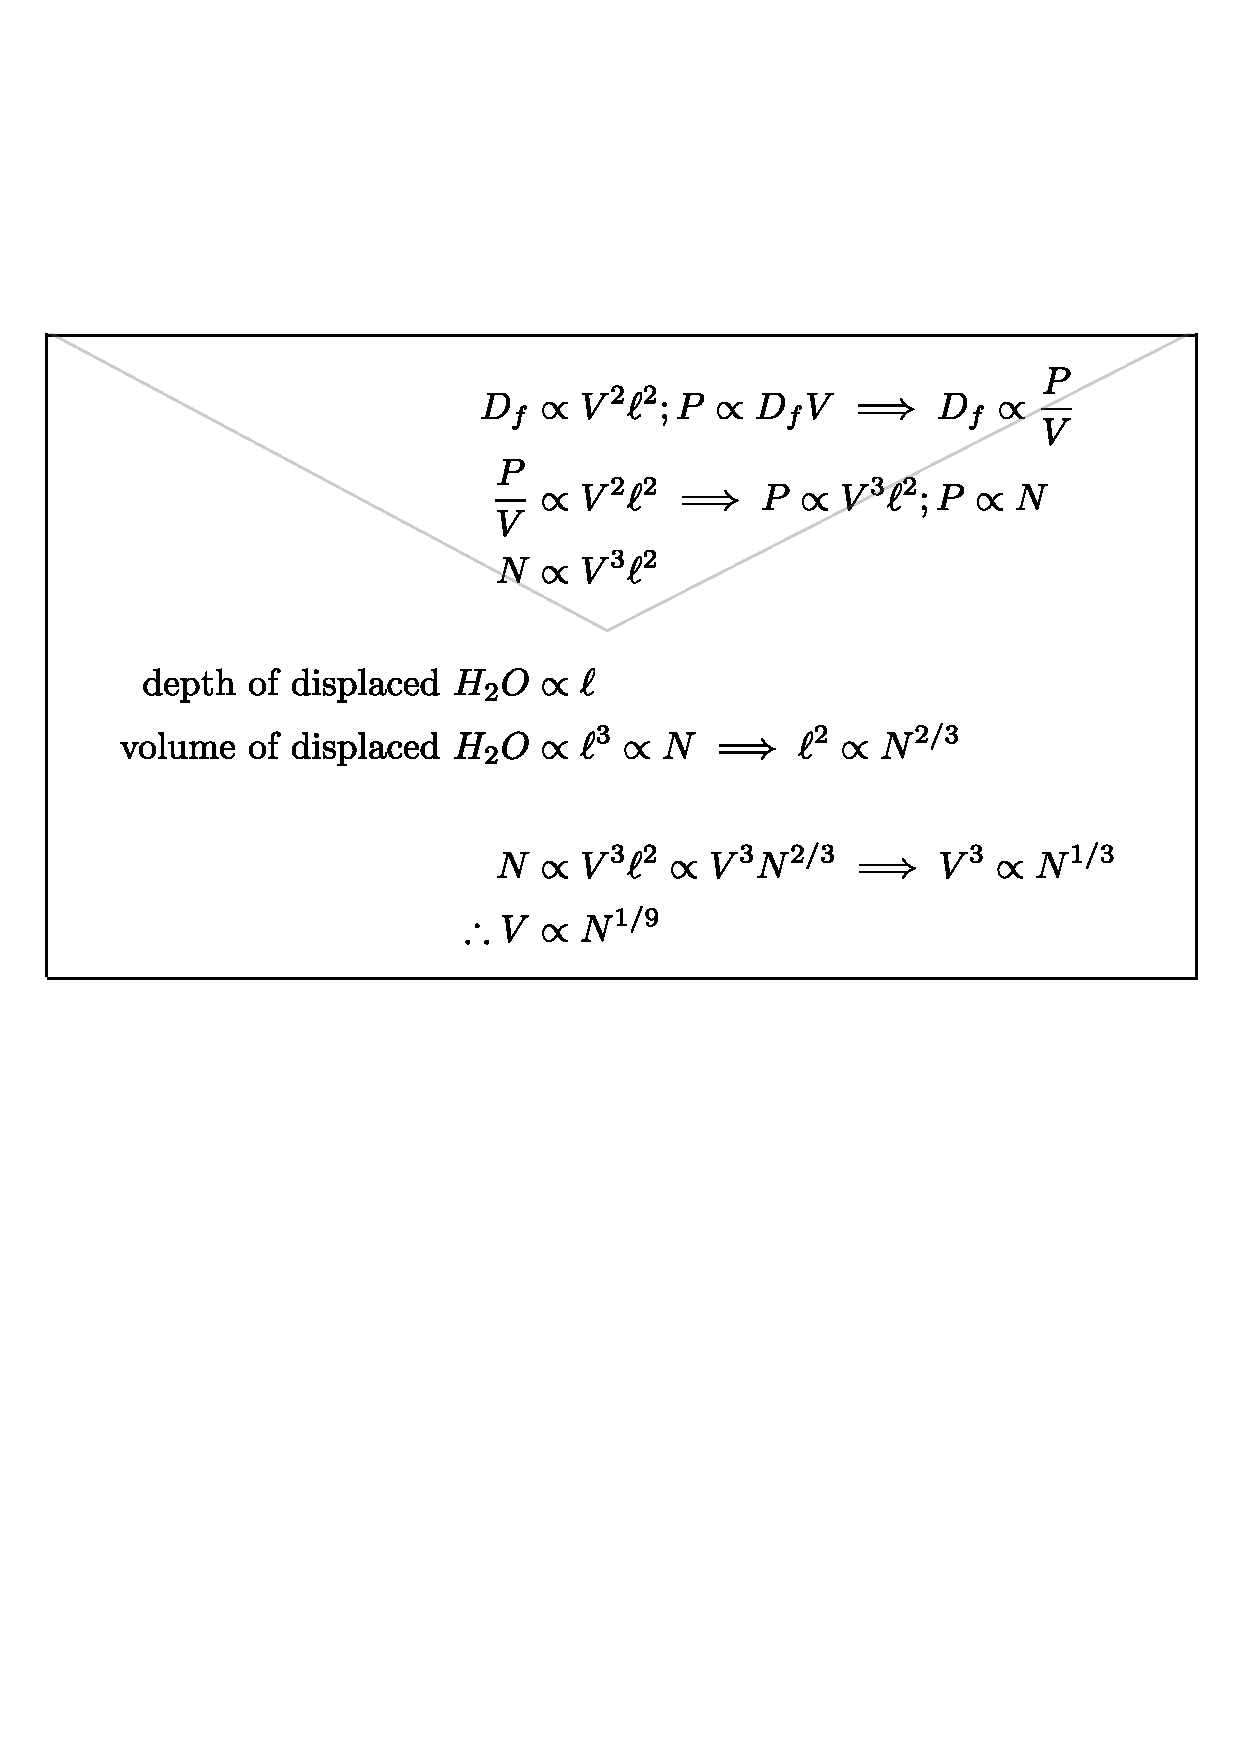
\includegraphics[width=\linewidth]{Q01/powerLawEnvelope.pdf}
  \caption{The above figure shows the back of the actual envelope on which the power law scaling of shell velocity, $V$, as a function of total oarspeople, $N$, was derived.}
  \label{fig:envelope}
\end{figure}

\section{Exercise 2}

\begin{figure}[h!]
  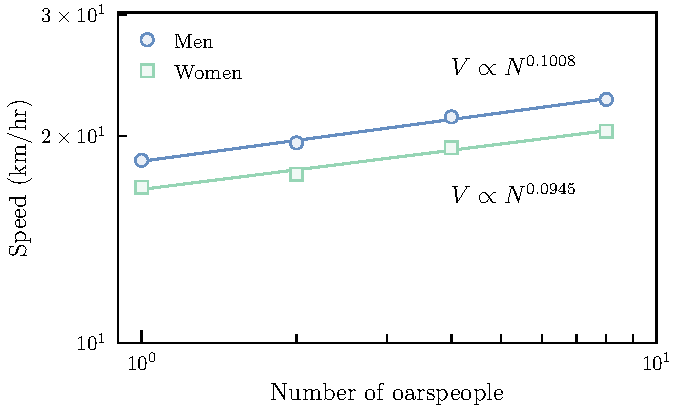
\includegraphics[width=\linewidth]{Q02/rowingPowerLaw.pdf}
  \caption{INSERT CAPTION}
  \label{fig:rowingPowerLawPlot}
\end{figure}



\section{Exercise 3}

\begin{figure}[h!]
  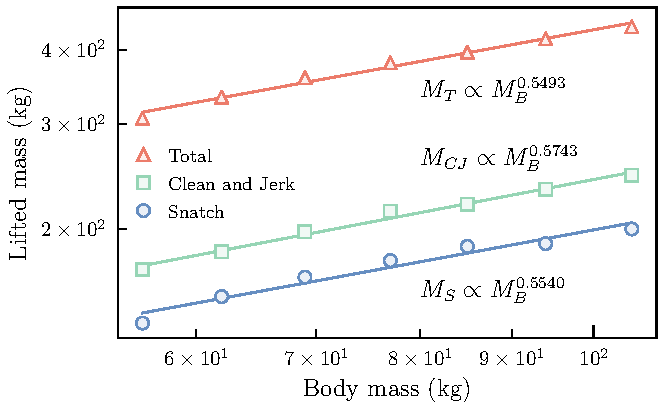
\includegraphics[width=\linewidth]{Q03/liftingPowerLaw.pdf}
  \caption{INSERT CAPTION}
  \label{fig:liftingPowerLawPlot}
\end{figure}

\begin{figure}[h!]
  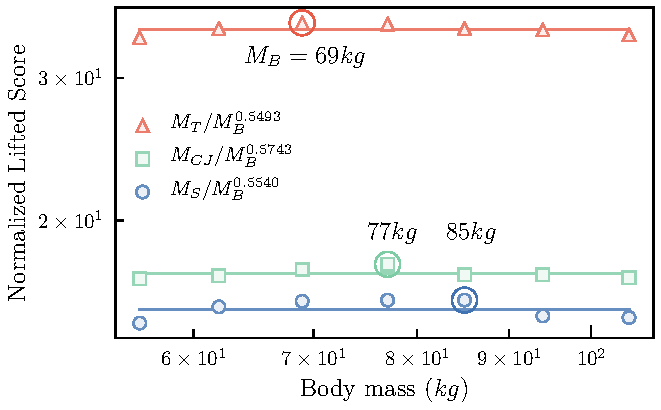
\includegraphics[width=\linewidth]{Q03/liftingPowerLawNormed.pdf}
  \caption{INSERT CAPTION}
  \label{fig:liftingPowerLawPlot}
\end{figure}

\section{Exercise 4}

\section{Exercise 5}

\section{Exercise 6}

\section{Exercise 7}

\begin{figure}[h!]
  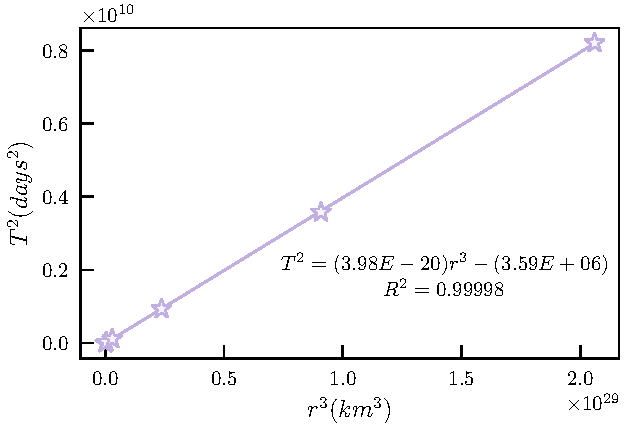
\includegraphics[width=\linewidth]{Q07/keplerLawPlot.pdf}
  \caption{INSERT CAPTION}
  \label{fig:keplerLawPlot}
\end{figure}

\section{Exercise 8}

\begin{figure}[h!]
  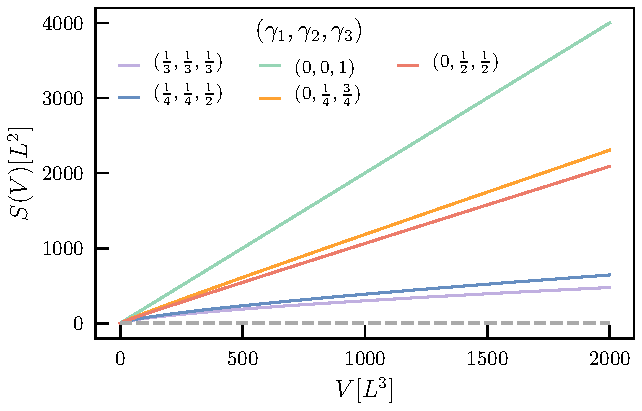
\includegraphics[width=\linewidth]{Q08/minecraftConvergence.pdf}
  \caption{INSERT CAPTION}
  \label{fig:minecraftConvergence}
\end{figure}

\end{document}